\chapter{Практические задания}

\section{Задание №1}

Представить следующие списки в виде списочных ячеек.

1. '(open close halph)\newline


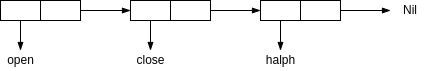
\includegraphics[scale=0.8]{img/1.1}

2. '((open1) (close2) (halph3))\newline

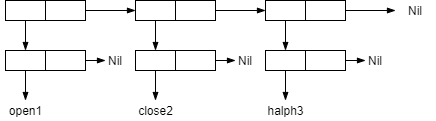
\includegraphics[scale=0.8]{img/1.2}

3. '((one) for all (and (me (for you))))\newline

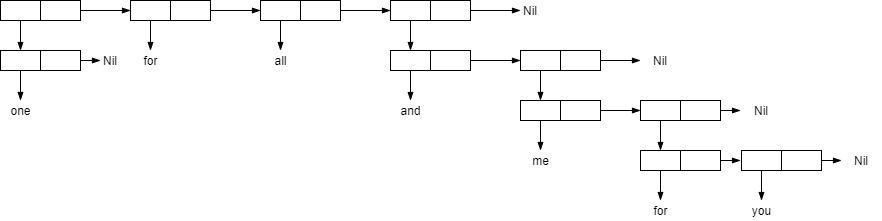
\includegraphics[scale=0.55]{img/1.3}

4. '((TOOL) (call))\newline

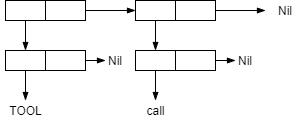
\includegraphics[scale=0.8]{img/1.4}

\clearpage
5. '((TOOL1) ((call2)) ((sell)))\newline

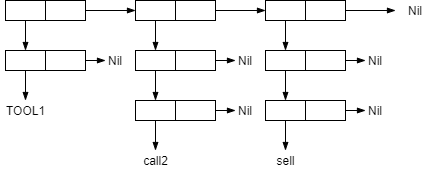
\includegraphics[scale=0.8]{img/1.5}

6. '(((TOOL) (call)) ((sell)))\newline

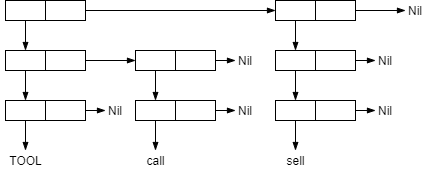
\includegraphics[scale=0.8]{img/1.6}

\section{Задание №2}

Используя функции $\text{CAR}$ и $\text{CDR}$, написать выражения,
возвращающие:
\begin{enumerate}
	\item второй элемент;

	\begin{lstlisting}[language=Lisp]
		(car (cdr '(a b c d))) => b
	\end{lstlisting}
	
	\item третий элемент;
	
	\begin{lstlisting}[language=Lisp]
		(car (cdr (cdr '(a b c d)))) => c
	\end{lstlisting}
	
	\item четвертый элемент.
	
	\begin{lstlisting}[language=Lisp]
		(car (cdr (cdr (cdr '(a b c d))))) => d
	\end{lstlisting}

\end{enumerate}

\section{Задание №3}

Что будет в результате вычисления выражений?

\begin{enumerate}
	\item Выражение:
	\begin{lstlisting}[language=Lisp]
		(caadr '((blue cube) (red pyramid)))
	\end{lstlisting}
	
	~~~~Результат: red
	
	\item Выражение:
	
	\begin{lstlisting}[language=Lisp]
		(cdar '((abc) (def) (ghi)))
	\end{lstlisting}
	
	~~~~Результат: Nil
	
	\item Выражение:
	
	\begin{lstlisting}[language=Lisp]
		(cadr '((abc) (def) (ghi)))
	\end{lstlisting}
	
	~~~~Результат: (def)
	
	\item Выражение:
	
	\begin{lstlisting}[language=Lisp]
		(caddr '((abc) (def) (ghi)))
	\end{lstlisting}
	
	~~~~Результат: (ghi)
\end{enumerate}

\section{Задание №4}

Напишите результат вычисления выражений:

\begin{lstlisting}[language=Lisp]
	(list 'Fred 'and 'Wilma) => (Fred and Wilma). 
	(list 'Fred '(and Wilma)) => (Fred (and Wilma))
	(cons Nil Nil) => (Nil . Nil) => (Nil)
	(cons T Nil) => (T . Nil) => (T)
	(cons Nil T) => (Nil . T)
	(list Nil) => (Nil)
	(cons '(T) Nil)	 => ((T) . Nil)	 => ((T))
	(list '(one two) '(free temp)) => ((one two) (free temp))
	
	(cons 'Fred '(and Willma)) => (Fred . (and Willma)) => (Fred and Willma)
	(cons 'Fred '(Wilma)) => (Fred .  (Willma)) => (Fred Willma)
	(list Nil Nil) => (Nil Nil)
	(list T Nil) => (T Nil)
	(list Nil T) => (Nil T)
	(cons T (list Nil)) => (cons T '(Nil)) => (T . (Nil)) => (T Nil)
	(list '(T) Nil) => ((T) Nil)
	(cons '(one two) '(free temp)) => ((one two) . (free temp))  => ((one two) free temp)
\end{lstlisting}


\section{Задание №5}

Написать лямбда-выражение и соответствующую функцию. Представить результаты в виде списочных ячеек.

1. Написать функцию (f ar1 ar2 ar3 ar4), возвращающую список: ((ar1 ar2) (ar3 ar4)).
\begin{lstlisting}[language=Lisp]
(defun f1 (ar1 ar2 ar3 ar4) (list (list ar1 ar2) (list ar3 ar4)))

(lambda (ar1 ar2 ar3 ar4) (list (list ar1 ar2) (list ar3 ar4)))
\end{lstlisting}

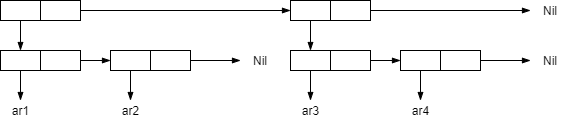
\includegraphics[scale=0.8]{img/1}

2. Написать функцию (f ar1 ar2), возвращающую ((ar1) (ar2)).
\begin{lstlisting}[language=Lisp]
(defun f (ar1 ar2) (list (list ar1) (list ar2)))

(lambda (ar1 ar2) (list (list ar1) (list ar2)))
\end{lstlisting}

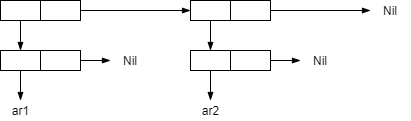
\includegraphics[scale=0.8]{img/2}

3. Написать функцию (f ar1), возвращающую (((ar1))).
\begin{lstlisting}[language=Lisp]
(defun f (ar1) (list (list (list ar1))))

(lambda (ar1) (list (list (list ar1))))
\end{lstlisting}

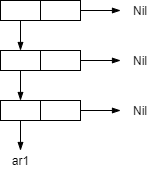
\includegraphics[scale=0.8]{img/3}


\chapter{Теоретические вопросы}

\section{Элементы языка: определение, синтаксис, представление в памяти}

Вся информация (данные и программы) в Lisp представляется в виде символьных
выражений --- S-выражений.

\vspace{4mm}
\begin{minipage}{0.92\linewidth}
		S-выражние ::= <атом>|<точечная пара>
\end{minipage}

Атомы:
\begin{itemize}
	\item символы --- синтаксически --- набор литер (букв и цифр), начинающийся
	с буквы;
	\item специальные символы \{T, Nil\} обозначают логические константы;
	\item самоопределимые атомы --- натуральные, дробные, вещественные
	числа и строки.
\end{itemize}

Более сложные данные --- точечные пары и списки (структуры).

Точечная пара ::= (<атом>. <атом>) 
| (<атом>, <точечная пара>)
| (<точечная пара>. <атом>)
| (<точечная пара>. <точечная пара>)

Список ::= <пустой список> | <непустой список>, где \newline
<пустой список> ::= () | Nil,\newline
<непустой список> ::= (<первый элемент>. <хвост>),\newline
<первый элемент> ::= <S-выражение>,\newline
<хвост> ::= <список>.


Синтаксически любая структура заключается в круглые скобки:
\begin{itemize}
	\item (A . B) -- точечная пара;
	\item (A) -- список из одного элемента;
	\item Nil или () -- пустой список;
	\item (A . (B . (C . (D ()))))) или (A B C D) -- непустой список;
	\item элементы списка могу являться списками: ((A)(B)(CD)).
\end{itemize}

Любая непустая структура Lisp в памяти представляется списковой ячейкой,
хранящей два указателя: на голову (первый элемент) и хвост (все остальное).

\section{Особенности языка Lisp. Структура программы. Символ апостроф}

Особенности языка Lisp:
\begin{itemize}
	\item символьная обработка данных;
	\item любая программа может интерпретироваться как функция с
	одним или несколькими аргументами;
	\item автоматизированное динамическое распределение памяти, которая
	выделяется блоками;
	\item бестиповый язык;
	\item программа может быть представлена как данные, то есть программа
	может изменять саму себя.
\end{itemize}

Символ апостроф --- сокращеное обозначение функции quote, блокирующей
вычисление своего аргумента.

\section{Базис языка Lisp. Ядро языка}

Базис языка --- минимальный набор конструкций и структур данных, с помощью
которого можно написать любую программу.

Базис Lisp образуют:
\begin{itemize}
	\item атомы;
	\item структуры;
	\item базовые функции;
	\item базовые функционалы.
\end{itemize}

Функцией называется правило, по которому каждому значению одного или нескольких  аргументов ставится в соответствие конкретное значение результата.

Функционалом, или функцией высшего порядка называется функция, аргументом или  результатом которой является другая функция.

Помимо базиса языка, ядро включает в себя наиболее часто используемые функции, не входящие в базис.

